\lstset{language=HTML}

\section{{\sys} policy model}
\label{sec:model}
{\sys} works on a browser that has already been augmented with IFC
enforcement based on taint tracking.
% Such an enforcement labels all objects internally.
It provides a framework that allows setting labels at
fine-granularity, thus expressing and enforcing rich policies. This
section explains the design of {\sys}. {\sys} prevents under-the-hood
exfiltration of sensitive data that has been provided to third-party
scripts for legitimate reasons. So, third-party scripts are not
trusted but code from the host domain is trusted.
{\sys}'s policies are agnostic to specific channels of leak.  However, 
current IFC enforcements in browsers track only explicit and implicit 
flows. Consequently, leaks over other channels such as timing and
memory-usage are currently out of scope. % As IFC enforcements improve 
% to cover more channels, {\sys}'s policies will extend to them as well.

\subsection{Policies as event handlers}

The first question in the design of {\sys} is who should specify
policies. Since the goal here is to prevent exfiltration of data by
third-party scripts and it is the developer of the host page who
bootstraps the inclusion of scripts and best understands how data on
the page should be used, it is natural and pragmatic to have the
developer specify policies, possibly as part of the page itself.

The next question is how the developer specifies policies. To answer
this, recall the two requirements identified in
Section~\ref{sec:overview} --- it should be possible to specify
different policies on different page elements and policies should be
allowed to include code that is executed on-the-fly to generate
labels. Considering the fact that sensitive data is usually
generated by input events, it is clear that policies should \emph{be}
page element-specific (trusted) code that is executed after events
have occurred (this code labels event-generated data). Fortunately,
web browsers provide exactly this abstraction in the form of event
handlers! So, the event-handling logic in web browsers is extended to
express {\sys} policies. This allows leveraging a lot of the existing
browser logic for event handler installation, parsing and event
dispatch in interpreting policies. The rest of this section explains
how this is done. 
% starting with a brief overview of event handling in web browsers.

% \medskip \noindent \textbf{Event handlers and event dispatch.}
% Browsers execute JavaScript functions, called event handlers, in
% response to input events like mouse clicks, key presses, and
% asynchronous network receives. Save for network receive events, every
% event has a \emph{target}, which is an element in the page's DOM where
% the event originated. For instance, if a button is clicked, the target
% of the ensuing event is the button. Code running on a page can add an
% event handler on any element on the page, listening for a specific
% event. When an event occurs, all handlers associated for that event
% with the event's target and the target's ancestors are triggered
% sequentially. This is called \emph{event dispatch.} The specific order
% in which handlers are triggered is not relevant for our purposes
% (although it is fairly interesting for IFC
% enforcement~\cite{csf15}). The whole process is bootstrapped by the
% static HTML of the page, which may contain JavaScript that is executed
% when the page loads initially, and this JavaScript installs the first
% set of event handlers.

% \medskip \noindent \textbf{Policy handlers.}
In {\sys}, policies are special event handlers, specified using a
special marker in the HTML source of the hosting page. These special
handlers, called \emph{policy handlers}, follow standard JavaScript
syntax, can be attached to any page element, listening for any event
and, like other handlers, are triggered every time the event is
dispatched on the element or any of its descendants. However, unlike
other handlers, the sole goal of policy handlers is to assign labels
to other sensitive objects, including the event being dispatched. To
allow the policy handlers to do this, the browser is slightly modified 
to afford these handlers two special privileges:
\begin{itemize}
\item Policy handlers can execute two new JavaScript API functions
  that set labels on other objects. No other JavaScript code can
  execute these two functions. These functions are described later.
\item During event dispatch all applicable policy handlers are executed
  before ordinary handlers. This ensures that labels are set before
  ordinary handlers (including those of third-party scripts) execute.
\end{itemize}
To maintain the integrity of the policies, policy handlers must be
included in the HTML source of the page directly. They \emph{cannot}
be installed dynamically by JavaScript code. Otherwise, third-party
scripts could install policy handlers that set very permissive labels.
Also, if a DOM element has a policy handler, third-party scripts are
disallowed from detaching that element or moving it elsewhere, as that 
can change the interpretation of the policy. Similarly, changing the
attributes of such an element is restricted.

\begin{figure}[tb]
  \centering 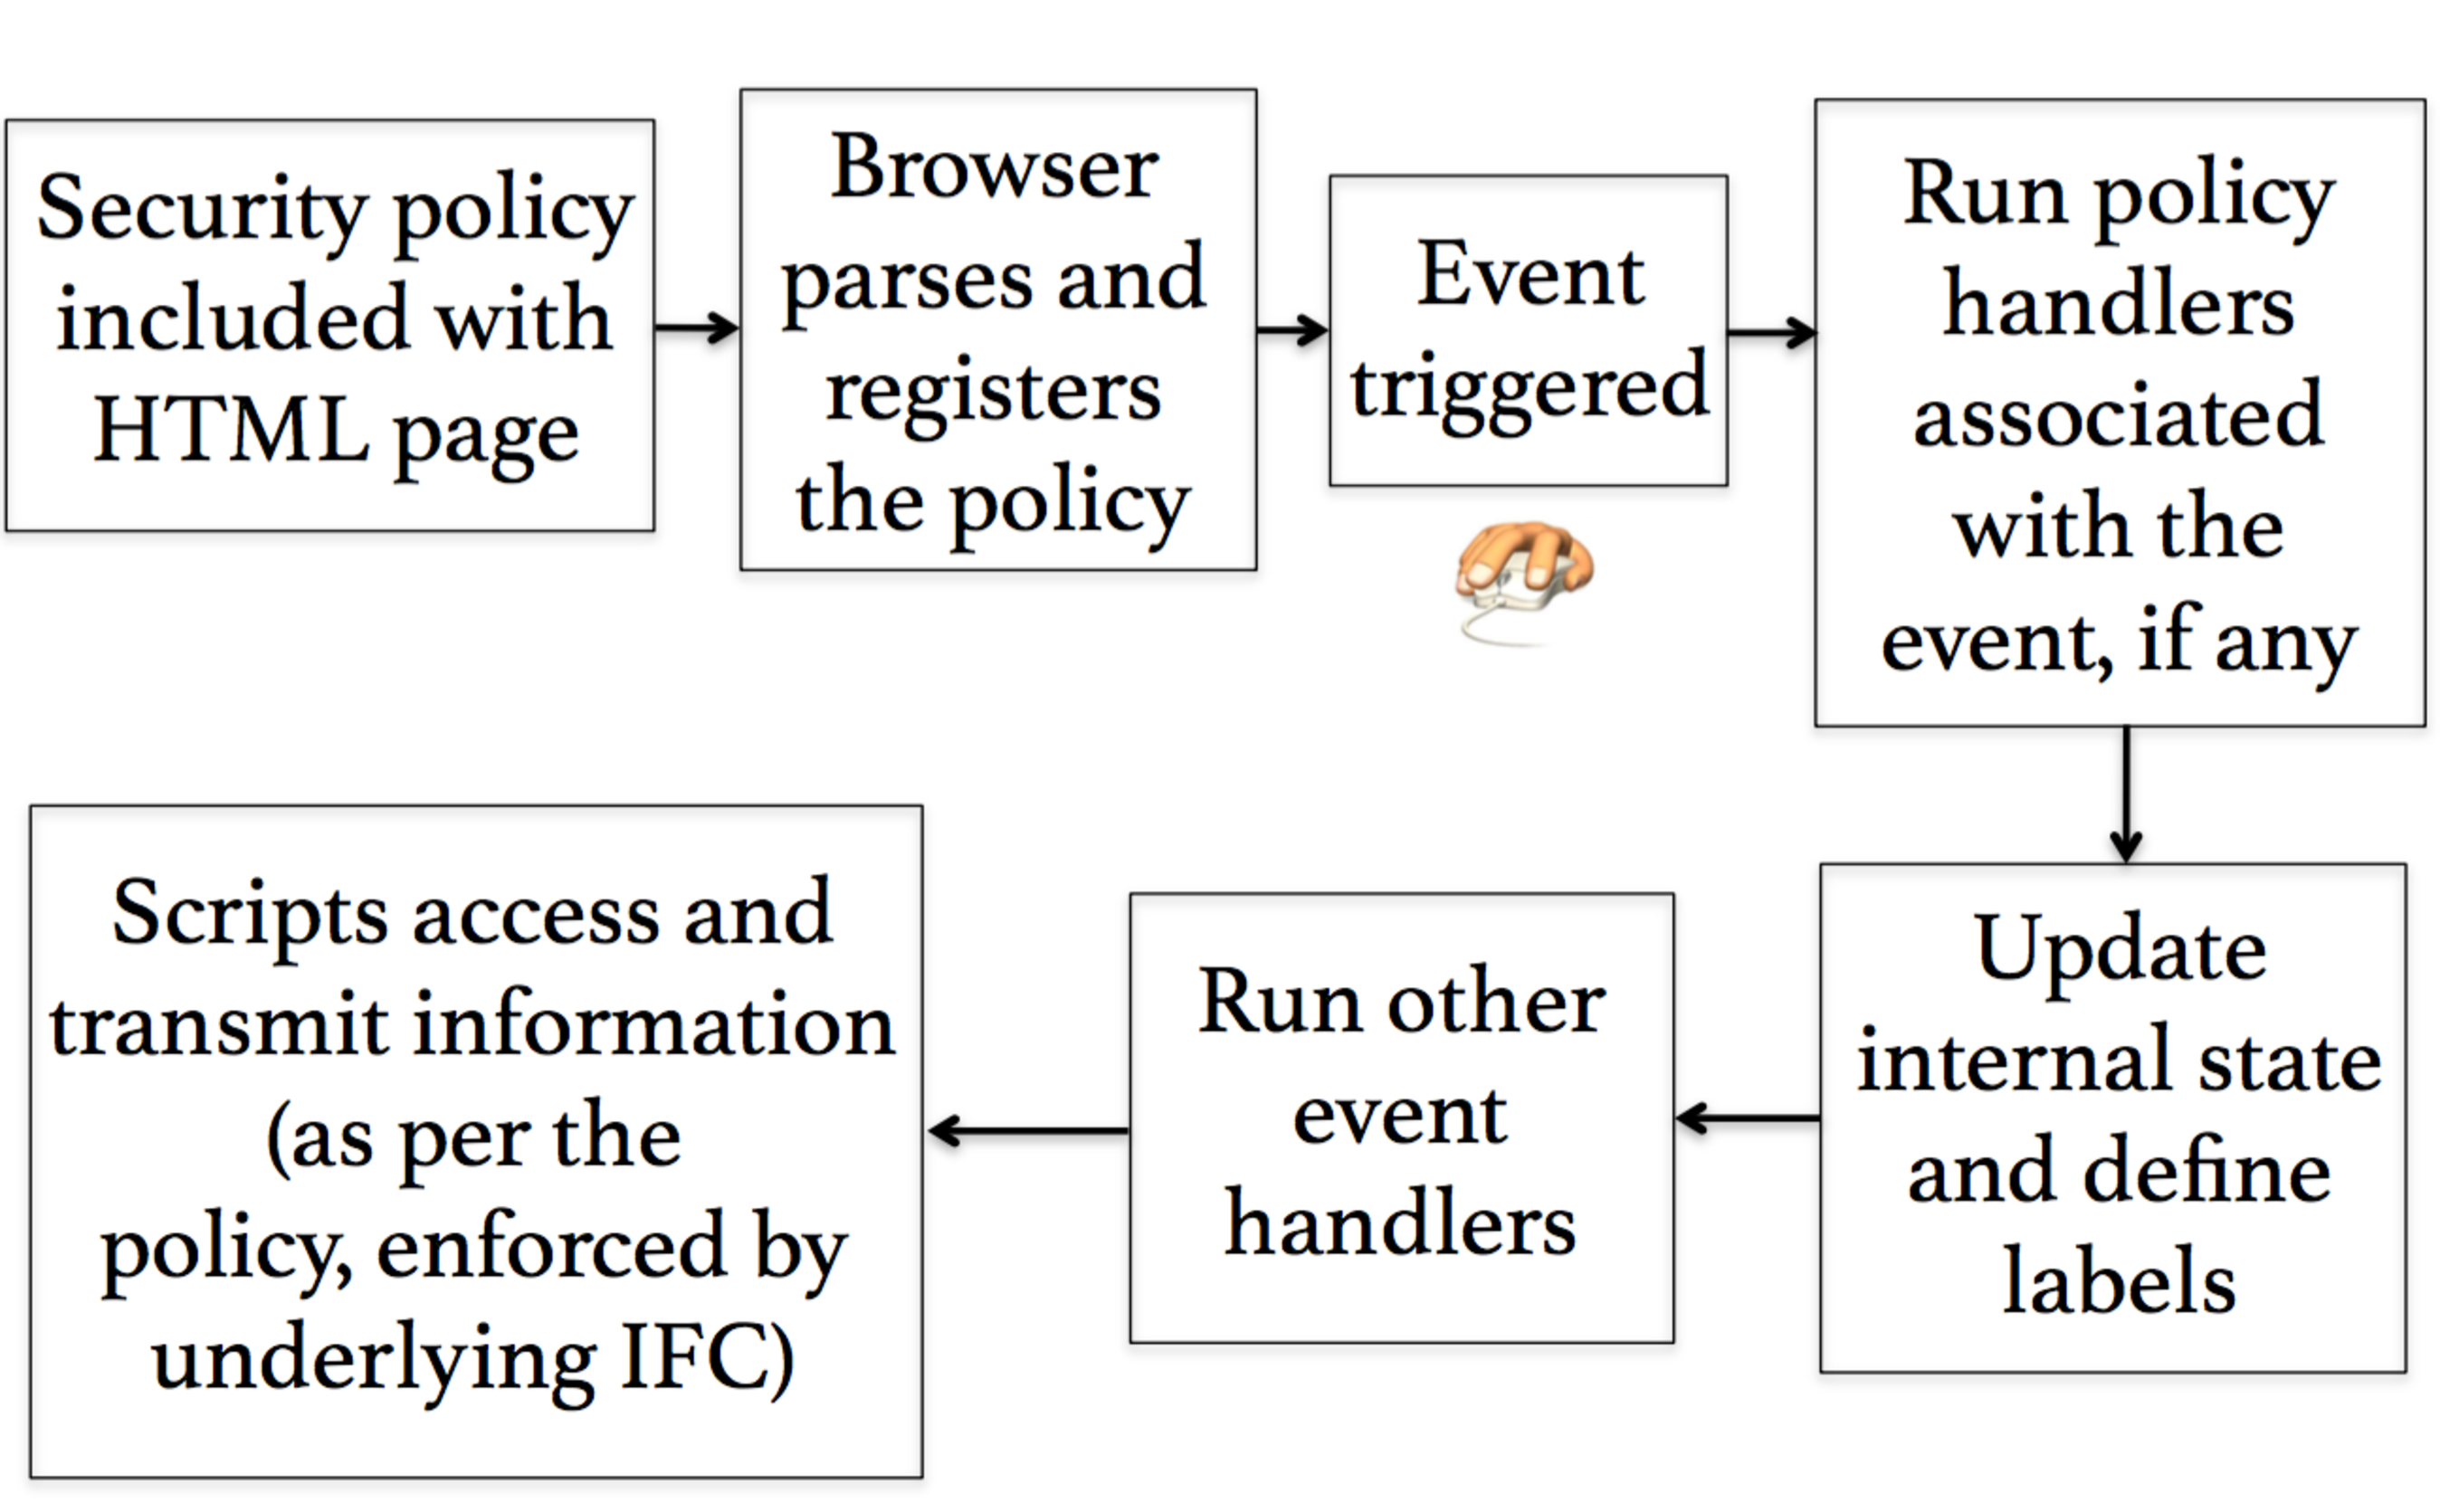
\includegraphics[width=8cm]{chapters/browser/webpol/Model.pdf} \caption{Workflow
  of the {\sys} policy model} \label{fig:model}
\end{figure}

Since different policy handlers can be associated with different
elements, Requirement~1 is satisfied.  Moreover, policy handlers are
ordinary JavaScript code, so they can also maintain local state in
private variables, thus satisfying Requirement~2. 

The workflow of policy interpretation in {\sys} is shown in
Figure~\ref{fig:model}. Briefly, the steps are:

\begin{enumerate}
\item The web page developer specifies the policy in the host HTML
  page in the form of special event handlers.
\item The browser parses the policy and registers its handlers (mostly
  like usual handlers, but with the two special privileges mentioned
  above).
\item When an event dispatches, listening policy handlers are
  executed first.
\item These policy handlers set labels on objects affected by the
  event, including the event object itself. They may also
  update any local state they maintain.
\item The remaining event handlers are dispatched as usual.
  The IFC enforcement in the browser enforces all labels that have
  been set by the policy handlers (during any prior event's dispatch),
  thus preventing any data leak in contravention of the labels.
\end{enumerate}

\subsection{Integration with the web browser}

{\sys} needs minor modifications to the browser to parse and interpret
policies and to expose additional JavaScript API functions to set
labels.

\medskip \noindent \textbf{HTML and event dispatch changes.}
{\sys} adds an HTML extension to differentiate policy code from other
JavaScript code. Concretely, the browser's parser is changed to
interpret any script file with the extension \texttt{.policy} included
directly in the host page as a policy. If such a \emph{policy script}
installs a handler, it is treated as a policy handler. Additionally, a
policy script can set labels on the page's global variables and DOM
elements (like password fields). If a script does this, it should be
included in the host page before third-party scripts that use those
variables. {\sys} also requires a small change to the browser's event
dispatch mechanism to execute policy handlers before other handlers.

\medskip \noindent \textbf{Label-setting APIs.}
{\sys} exposes two new JavaScript API functions to set labels. These
functions can be called only by the policy code in \texttt{.policy}
files and handlers installed by such files (the browser is modified to
enforce this).

The function \texttt{setLabel(label)} sets the label of the object on
which it is called to \texttt{label}. As explained
earlier, \texttt{label} can be \texttt{public}, a domain name,
or \texttt{local} (the default is \texttt{public}). Once an object's
label is set, it is enforced by the underlying IFC enforcement. The
special label \texttt{HOST} is a proxy for the domain of the host
page.

The function \texttt{setContext(label)} can be called only on an event
object. It restricts the \emph{visibility} of the event to
label \texttt{label} and higher. In simple terms, if \texttt{label} is
a domain, then only that domain can ever learn that this event
occurred, whereas if \texttt{label} is \texttt{local}, then no domain
can ever learn that this event occurred. Technically, this is
accomplished by setting the $\pc$ of the 
event handlers running during the dispatch to \texttt{label}, which
ensures that their side-effects (writes to DOM and network
communication) are labeled \texttt{label} or higher.

As opposed to \texttt{setLabel}, which makes individual data objects
(like password fields) private, \texttt{setContext} makes the
\emph{existence} of an event private. This is useful.
For instance, clicking on the ``politics'' section of a news feed
might indicate that the user is interested in politics, which may be
private information, so the page may want to hide even the existence
of click events from third-party scripts. (The distinction between the
privacy of event content and event occurrence has been previously
described by Rafnsson and Sabelfeld~\cite{Rafnsson-csf13}.)

